\section*{REGRESSION}\label{regression}
The ship power data is split into a train and a test part. In the time
series the samples are not independent, which means that splitting the
data into a train and test set, should not be done randomly. It can be
seen in Fig.\ref{fig:random_train_test} that a random test set
would almost reproduce the training set perfectly, which would be a poor
test, as the model has already seen very similiar data before. Instead
it is very important that observations from the training set occur
before their corresponding test set. Fig.\ref{fig:train_test}
shows the train-test-split of the present data, where the last 20\% of
the data is used for testing. Due to the same reasoning,
cross-validation on a rolling basis is used for parameter tuning as seen
in Fig.\ref{fig:rolling_basis}.
\begin{figure}[H]
\begin{center}\includegraphics[width = 0.95\textwidth]{figures/random_figures/train_test.pdf}\end{center}
\vspace{-0.7cm}
\caption{Using a random test set should not be used as this almost reproduces the train set.}
\label{fig:random_train_test}
\end{figure}
\begin{figure}[H]
\begin{center}\includegraphics[width = 0.95\textwidth]{figures/train_test.pdf}\end{center}
\vspace{-0.7cm}
\caption{Data is split into a train and test part}
\label{fig:train_test}
\end{figure}
\begin{figure}[H]
\begin{center}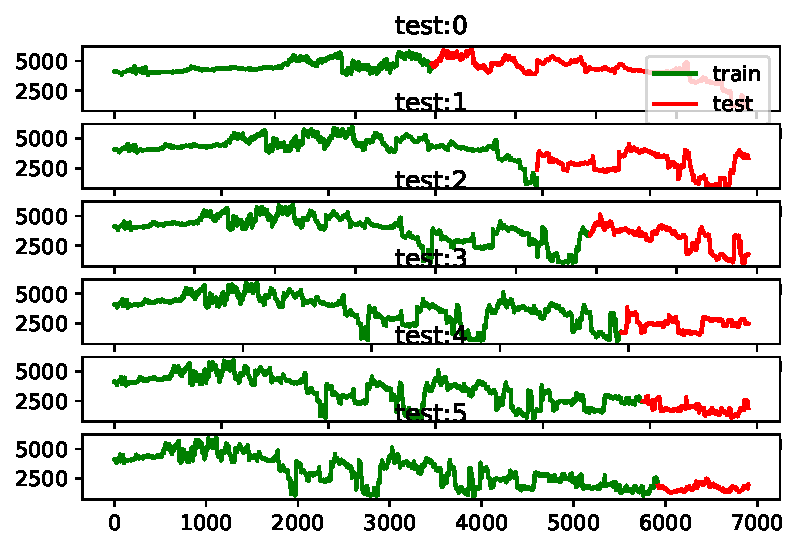
\includegraphics[width = 0.95\textwidth]{figures/rolling_basis.pdf}\end{center}
\vspace{-0.7cm}
\caption{Cross-validation on a rolling basis}
\label{fig:rolling_basis}
\end{figure}
